\chapter{TINJAUAN PUSTAKA}

% Ubah konten-konten berikut sesuai dengan isi dari tinjauan pustaka
\section{Hasil penelitian/perancangan terdahulu}

\subsection{\emph{PPE detector: a YOLO-based architecture to detect personal protective equipment (PPE) for construction Sites}}

Md. Ferdous dan Sk. Md. Masudul Ahsan pada bulan April 2022 lalu melakukan penelitian berjudul "PPE detector: a YOLO-based architecture to detect personal protective equipment (PPE) for construction Sites" dimana mereka membuat sistem pendeteksi APD otomatis berbasis Visi Komputer. Sedangkan untuk algoritma deteksi yang digunakan, penelitian ini menggunakan arsitektur \emph{anchor-free} YOLO --- yaitu YOLO versi X atau YOLOX secara spesifik. Penelitian ini menggunakan dataset bernama "CHVG Dataset" dimana CHVG merupakan kependekan dari \emph{Color Hardhat Vest Glass} yang merupakan deskripsi dari isi dari dataset itu sendiri. Dataset tersebut merupakan salah satu \emph{output} dari penelitian ini yang dibuat sendiri oleh para penulis dengan cara menambahkan dan menggabungkan data dari dataset penelitian-penelitian sebelumnya yang terkait serta sebagai pengembangan dari dataset penelitian-peneli- tian sebelumnya tersebut. Sistem deteksi yang dibuat oleh penelitian ini masih menerima \emph{input} dalam bentuk file gambar atau foto dan belum \emph{real-time} menggunakan kamera webcam yang menangkap citra video namun hasil prediksi dari model YOLOX sudah ditampilkan pada antarmuka sistem. Dari hasil pengujian yang dilakukan, didapatkan rata-rata mAP terbesarnya yaitu 89,84\% yang dihasilkan oleh model dengan jenis YOLOX-m \cite{ferdous_ahsan_2022}.

\subsection{Rancang Sistem Pendeteksi Alat Pelindung Diri (APD) Berbasis \emph{Image Prosessing}}

Miftachul Ulum bersama 3 rekannya pada tahun 2021 melakukan penelitian tentang peran-
cangan sistem pendeteksi Alat Pelindung Diri (APD) antara lain helm, kacamata, dan masker
dengan menerapkan metode CNN yang berbasis image processing. Sistem deteksi yang dirancang pada penelitian ini masih menerima input hanya dalam bentuk file gambar (tidak \emph{real-time}) yang berasal dari hasil tangkapan citra webcam. Selain itu hasil prediksi dari model yang digunakan tidak divisualisasikan langsung pada antarmuka sistem dan hanya bergantung pada \emph{buzzer} yang sudah diprogram untuk menyala jika terdeteksi APD tidak lengkap.
Dari hasil pengujian, didapatkan akurasi keberhasilan 75\% dengan klasifikasi objek yang menggunakan APD lengkap,
APD tidak lengkap, dan tidak menggunakan APD. Pada penelitian ini ditemukan bahwa komponen APD kacamata lebih sering tidak terdeteksi dibanding komponen APD lainnya yang
disebabkan oleh pantulan cahaya dari kacamata yang dapat mengganggu proses penangkapan gambar. Selain itu pada penelitian ini juga ditemukan bahwa kemampuan kamera dan komputer
akan memengaruhi kinerja sistem secara keseluruhan \cite{miftachul_2021}.

\section{Teori/Konsep Dasar}

\subsection{Alat Pelindung Diri}
\label{apd}

Dalam setiap pekerjaan, seorang pekerja memiliki kemungkinan mengalami kecelakaan yang mempengaruhi kondisi kesehatannya. Keselamatan dan kesehatan kerja berkaitan dengan alat kerja, proses pengolahan, dan bahan, lingkungan kerja dan proses melakukan pekerjaannya. Kecelakaan merupakan kejadian yang tidak terduga dan tidak pernah diharapkan karena dapat menimbulkan kerugian materil dan juga penderitaan mulai dari penderitaan yang ringan sampai dengan penderitaan yang paling berat \cite{anizar2012}.

Seperti diketahui, ada 5 tahapan yang mencakup upaya pencegahan kecelakaan dalam hierarki pengendalian risiko, yaitu: tahap eliminasi, substitusi, tahap engineering, tahap administrasi dan terakhir alat pelindung diri. Penggunaan alat ini bukanlah pilihan pertama melainkan yang terakhir jika 4 langkah tersebut belum dilakukan atau telah dilakukan namun masih terdapat bahaya yang mengganggu status kesehatan tenaga kerja. Penggunaan alat ini akan menimbulkan ketidaknyamanan pekerja namun mampu mencegah atau mengurangi resiko penyakit akibat kerja dan kecelakaan kerja \cite{k3ptglobal}.

Alat Pelindung Diri selanjutnya disingkat APD adalah
suatu alat yang mempunyai kemampuan untuk melindungi
seseorang yang fungsinya mengisolasi sebagian atau
seluruh tubuh dari potensi bahaya di tempat kerja.
Penggunaan APD diatur dalam Peraturan Menteri Tenga Kerja
dan Transmigrasi Republik Indonesia NOMOR PER.08/MEN/VII/2010
tentang ALAT PELINDUNG DIRI (dan Transmigrasi Republik Indonesia, 2010a) \cite{suratkementriantenagakerja}.

\subsection{Peraturan Menteri Tenaga Kerja dan Transmigrasi Republik Indonesia tentang Alat Pelindung Diri}
\label{peraturanapd}

Peraturan Menteri Tenaga Kerja dan Transmigrasi (Kemnakertrans) Republik Indonesia NOMOR PER.08/MEN/VII/2010 mengatur tentang alat pelindung diri.
Peraturan ini meliputi pihak - pihak yang terlibat, kewajiban penyediaan APD, peralatan yang termasuk APD, dan karakteristik tempat
yang diwajibkan APD \cite{suratkementriantenagakerja}. Pada pasal 3 ayat 1, disebutkan alat - alat yang termasuk sebagai alat pelindung diri
yaitu :

\begin{enumerate}[nolistsep]
  \item pelindung kepala
  \item pelindung mata dan muka
  \item pelindung telinga
  \item pelindung pernapasan beserta kelengkapannya
  \item pelindung tangan
  \item pelindung kaki
\end{enumerate}

\subsection{Peraturan Menteri Pekerjaan Umum dan Perumahan Rakyat tentang Pedoman Sistem Manajemen Keselamatan Konstruksi}
\label{sec:permenpu_smkk}

\par Peraturan Menteri Pekerjaan Umum dan Perumahan Rakyat NOMOR : 21/PRT/M/2019 mengatur Pedoman Sistem Manajemen Keselamatan Konstruksi.
Petaturan ini meliputi ketentuan umum untuk SMKK (Sistem Manajemen Keselamatan Konstruksi), Konseptual SMKK, elemen SMKK, penerapan, penyedia jasa, pelaksanaan pekerjaan konstruksi,  dan beberapa aturan lainnya yang menyinggung ketentuan Kesehatan Keselamatan Kerja (K3) pada konstruksi. Pada pasal 1 untuk ketentuan umum dimana pada ayat ke 10 menyebutkan adanya Pengawas Pekerjaan Konstruksi yang merupakan tim pendukung yang ditunjuk oleh Pengguna Jasa yang bertanggung jawab pada pengawasan Pekerjaan Konstruksi dan pemenuhan terhadap norma, standar, prosedur, dan kriteria \cite{permen21prtm2019pedomansistemmanajemenkeselamatankonstruksi}.

\subsection{Visi Komputer}
\label{sec:visikomputer}

\par Manusia bisa dengan mudahnya memahami struktur tiga dimensi yang ada di sekitarnya. Kita dapat mengetahui bahwa
sebuah balok memiliki ketebalan atau sebuah pot bunga yang memiliki isi. Kita juga dapat memahami benda yang semi transparan
seperti kantong plastik dimana cahaya matahari dapat menembus lembaran plastik tersebut. Lalu saat kita mengamati suatu kumpulan
barang - barang di gudang, kita juga dapat dengan mudahnya menentukan nama dari barang tersebut dan lokasinya. Begitu juga saat
mengamati foto keluarga yang terdiri dari banyak individu dimana kita dapat membedakan antara satu dengan yang lainnya bahkan hingga
emosi yang mereka perlihatkan lewat raut wajahnya. Peneliti sudah melakukan pengembangan untuk metode pengenalan visual seperti pada
manusia untuk komputer yang dimana bidangnya disebut sebagai \emph{Computer Vision} (Visi Komputer). Tetapi untuk mencapai titik dimana
komputer memiliki kemampuan untuk yang sama dengan manusia seperti dapat menghitung jumlah binatang yang ada dalam suatu gambar masih menjadi
sesuatu yang sulit. Hal ini dikarenakan bidang visi komputer ini merupakan bentuk \emph{inverse problem} dimana kita berusaha untuk menarik
suatu kesimpulan untuk suatu solusi tetapi informasi yang dimiliki sangat terbatas. Beberapa solusi yang memungkinkan untuk menyelesaiakan
permasalah visi komputer ini yaitu antaralain dengan penyelesaian secara fisika atau perhitungan probabilitas \cite{szeliski2010computer}.

\par Dalam visi komputer, kita berusaha untuk memahami dunia yang ditangkap dalam satu gambar atau lebih dan meniru ulang setiap detil nya seperti
bentuk, pencahayaan, dan pewarnaan. Manusia dapat dengan mudahnya memahami detail - detail tersebut sedangkan algoritma visi komputer
akan sering mengalami \emph{error} \cite{margaret2008mind}.

\par Visi Komputer adalah bidang ilmu yang mempelajari cara untuk memproses gambar teru- tama dalam meniru
kemampuan manusia dalam melihat. Kemampuan seperti rekognisi wajah hingga bentuk kemampuan lain yang bahkan
melebihi kemampuan manusia. Kebanyakan riset dari bidang visi komputer di \emph{deep learning} berfokus pada
pengenalan objek atau deteksi. Bentuknya dari pengenalan atau deteksi ini bisa meliputi membuat log atau laporan
objek apa saja yang ada dalam gambar hingga memberi penandaan pada objek yang terdeteksi \cite{Goodfellow-et-al-2016}.

\subsection{\emph{Object Detection}}
\label{sec:objectdetection}

\par Untuk dapat memahami konsep deteksi objek, selain menyelesaikan klasifikasi kelas dari objek yang diamati, kita juga harus dapat
menentukan lokasi dari objek yang diamati secara akurat dalam gambar yang sedang diamati. Proses penentuan lokasi sekaligus menentukan
klasifikasi kelas untuk menentukan "nama" dari objek yang diamati inilah yang disebut sebagai \emph{Object Detection} \cite{felzenszwalb2010object}.

\par Manfaat dari \emph{Object Detection} yaitu dapat memberikan informasi terkait suatu gambar atau video agar bisa lebih dipahami yang lalu bisa dimanfaatkan
untuk berbagai bentuk aplikasi. Penelitian di bidang \emph{Object Detection} ini pada umumnya berjalan di area \emph{neural network} atau sistem \emph{machine learning}
yang lalu juga termasuk pembuatan algoritma \emph{neural network} untuk teknik deteksi objek. Tetapi deteksi pada suatu gambar memiliki banyak
hal yang perlu dipertimbangkan seperti arah sudut pandang, pencahayaan, objek yang menghalang, dan hal lainnya yang membuat
deteksi objek dengan prediksi lokasi akurat semakin sulit untuk dilakukan \cite{zhao2019object} \cite{girshick2014rich}.

\par Proses penyelesain deteksi objek biasanya dilakukan dalam 3 tahap yaitu pemilihan wila- yah informatif, ekstraksi fitur, dan
klasifikasi.

\par Ada kemungkinan bahwa terdapat lebih dari satu objek yang ada dalam satu gambar yang akan dilakukan proses deteksi objek dan
juga berkemungkinan memiliki ukuran yang berbeda - beda. Pada tahap inilah dilakukan pemilihan region atau wilayah dengan melakukan \emph{scanning} pada gambar tersebut mulai
dari bagian awal gambar hingga akhir yang dimana merupakan metode yang sangat menguras energi dan memiliki banyak kelemahan \cite{zhao2019object}.

\par Tahap ekstraksi fitur kelas berguna untuk membedakan objek - objek yang berbeda dari gambar yang sedang diamati dimana kita perlu
memilah - milah "fitur" visual yang dapat memberi kita informasi yang dapat diapahami. Terdapat beberapa metode berbeda yang dilakukan
untuk mendapatkan fitur yang membantu untuk mengenali objek tersebut seperti SIFT, HOG, dan Haar-like \cite{zhao2019object}. Tetapi pada \emph{Convolutional Neural Network}
proses ekstraksi fitur nya dilakukan pada \emph{neural network}-nya juga yang akan dijelaskan pada Subbab~\ref{sec:convolutionalneuralnetwork}.

\par Klasifikasi berguna untuk mengenali objek yang ada pada gambar dengan kategori - kategori. Juga sudah terdapat beberapa metode
klasifkasi yang biasa digunakan seperti \emph{Supported Vector Machine}, AdaBoost, dan \emph{Deformable Part-based Model} \cite{zhao2019object}.

\subsection{\emph{Convolutional Neural Network} (CNN)}
\label{sec:convolutionalneuralnetwork}

\par \emph{Convolutional Neural Network} adalah metode deep learning yang didesain untuk rekognisi pada data dua
dimensi yang dimana umumnya berupa gambar visual (tetapi tidak harus berupa gambar) dan untuk klasifikasi.
Convolutional Neural Network memiliki kedalaman jaringan yang tinggi sehingga juga bisa termasuk sebagai \emph{Deep Neural Network}.
Jika dibandingan dengan \emph{Multilayer Perceptron} atau MLP, kemampuan CNN untuk klasifikasi citra lebih baik dibandingkan dengan MLP karena MLP tidak memiliki
kemampuan untuk menyimpan \emph{spatial information} dari gambar dimana satu \emph{pixel} pada gambar dianggap sebagai satu fitur
terpisah atau independen \cite{putra2016klasifikasi}. \emph{Convolutional Neural Network} adalah bentuk \emph{deep neural network} yang tidak hanya
sekadar memiliki banyak \emph{layer} seperti konsep \emph{deep learning} tetapi juga meniru bagaimaimana cara otak manusia mengenali sebuah gambar \cite{kim2017convolutional}. Pada arsitektur CNN, terdapat beberapa jenis layer yaitu \emph{Convolution Layer, Subsampling Layer,
  Fully Connected Layer}, dan \emph{Activation Layer}.

\subsection{\emph{You Only Look Once} (YOLO)}
\label{sec:youonlylookone}

\emph{You Only Look Once} atau YOLO adalah algoritma \emph{multi object detection} yang sangat cepat yang dicetuskan oleh Redmot et al pada tahun 2015 lewat buku mereka \emph{You Only Look Once: Unified, Real-Time Object Detection} \cite{redmon2016you}. \emph{Convolutional Neural Network} menjadi basis dari sistem deteksi YOLO ini. YOLO melakukan deteksi objek dengan menganggap nya sebagai permasalahan regresi tunggal yang diambil langsung dari \emph{pixel - pixel} yang ada di gambar menjadi \emph{bounding box} penanda dari koordinat - koordinat dan probabilitas dari klasifikasinya. Dengan begitu hanya perlu dilakukan satu kali pengecekan pada gambar untuk melakukan deteksi atau indentifikasi \cite{redmon2016you}. YOLO menggabungkan beberapa komponen dari teksi objek menjadi satu neural network yang dimana menggunakan fitu-fitur dari seluruh bagian gambar untuk memprediksi tiap \emph{bounding box} sekaligus melakukan prediksi untuk semua \emph{bounding box} di semua tipe klasifikasi yang ada. Desain dari YOLO ini memungkinkan untuk melakukan \emph{end to end training} dan kecepatan deteksi \emph{real time}.

\par Model YOLO (You Only Look Once) adalah pendeteksi objek \textit{single stage}. Bingkai gambar ditampilkan melalui \emph{\textit{Backbone}}, fitur digabungkan dan dicampur di \emph{\textit{Neck}}, dan kemudian diteruskan ke \emph{\textit{Head}} jaringan di mana YOLO memprediksi lokasi \emph{\textit{bounding box}}, kelas \emph{\textit{bounding box}}, dan objek \emph{\textit{bounding box}}. YOLO menggunakan pasca-pemrosesan melalui NMS untuk sampai pada prediksi akhirnya. Struktur jaringan tersebut ditunjukkan pada Gambar~\ref{fig:strukturyolo} \cite{strukturyolo}.

\begin{figure}[ht]
  \centering
  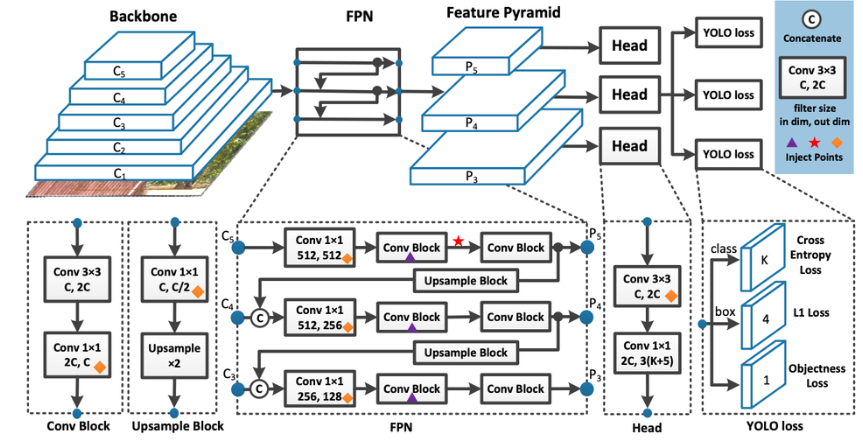
\includegraphics[width=0.85\textwidth]{gambar/arsitektur_yolo.png}
  \caption{Struktur Jaringan YOLO}
  \label{fig:strukturyolo}
\end{figure}

\par Sistem dari YOLO sendiri membagi input gambar menjadi grid S x S. Grid disini perannya untuk nanti yaitu jika grid tertentu menjadi pusat dari objek maka grid tersebut yang nantinya berguna untuk deteksi objek tadi.

\par Setiap grid memprediksi tiap bound box dan nilai kemungkinan klasifikasi atau \emph{confidence score} dari \emph{bounding box} tersebut. Nilai tersebut mewakili seberapa "yakin" model akan objek yang terdeteksi di bounding box dan seberapa akurat prediksinya.

\par Terdapat lima nilai prediksi yang ada pada tiap bounding box yaitu : x, y, w, h, dan \emph{confidence}. X dan Y mewakili pusat dari bounding box. W dan H mewakili \emph{Weight} dan \emph{Height} diprediksi relatif dari seluruh gambar. Lalu \emph{confidence score} sendiri mewakili IOU antara \emph{predicted box} dan \emph{ground truth box} \cite{redmon2016you}.

\subsection{YOLOv7}
\label{subsec:yolov7}

\par YOLOv7 adalah YOLO resmi versi terbaru yang dibuat oleh penulis asli arsitektur YOLO, melebihi semua versi YOLO sebelumnya dan model deteksi objek lainnya dalam hal kecepatan dan akurasi \cite{wang2022yolov7}. YOLOv7 meningkatkan kecepatan dan akurasi dengan memperkenalkan beberapa reformasi arsitektur. Mirip dengan \textit{Scaled} YOLOv4, YOLOv7 tidak menggunakan \textit{backbone pretrained} ImageNet. Sebaliknya, model dilatih menggunakan dataset COCO sepenuhnya. Kesamaan bisa diekspektasi karena YOLOv7 ditulis oleh penulis yang sama dari \textit{Scaled} YOLOv4 \cite{yolov7explain}.

Perubahan besar yang telah diperkenalkan pada makalah YOLOv7 salah satunya adalah reformasi arsitektur yaitu dengan adanya E-ELAN (\textit{Extended Efficient Layer Aggregation Network}) dan \textit{Model Scaling} untuk Model Berbasis Rangkaian. E-ELAN (\textit{Extended Efficient Layer Aggregation Network}) adalah blok komputasi di bagian \textit{Backbone} YOLOv7. Hal tersebut mendapatkan inspirasi dari penelitian sebelumnya tentang efisiensi jaringan. Ini telah dirancang dengan menganalisis faktor-faktor berikut yang memengaruhi kecepatan dan akurasi yaitu \textit{memory access cost, I/O channel ratio, element wise operation, activations}, dan \textit{gradient path}. Secara sederhana, arsitektur E-ELAN memungkinkan \textit{framework} untuk belajar lebih baik. Ini didasarkan pada blok komputasi ELAN \cite{yolov7explain}.